\chapter{}\label{ch:auf3}
In der bisherigen Darstellung gingen wir von einem bürstenlosen Gleichstrommotor mit der Polpaarzahl $ Z_{P} = 1 $ aus. Häufig werden jedoch Motoren mit höheren Polpaarzahlen verwendet. In dieser Aufgabe betrachten wir nun den Fall einer höheren Polpaarzahl, d.h. $ Z_{P} > 1$.

\section{}\label{sec:3a}
Es soll nun als erstes der Verlauf der digitalen Hallsensorsignale mit einer Polpaarzahl $ Z_{P} = 2 $ in einem Diagramm für eine volle Umdrehung des Rotors dargestellt werden.
Die Abbildung \ref{fig:3a:hall} zeigt ein Impulsdiagramm, welches nun die Hallsensorsignale für einen BLDC mit der Polpaarzahl $ Z_{P} = 2 $ dargestellt, ebenfalls bei einer vollen Umdrehung des Rotors im Rechtslauf.
\begin{figure}[h]
	\centering
	% This file was created by matlab2tikz.
%
%The latest updates can be retrieved from
%  http://www.mathworks.com/matlabcentral/fileexchange/22022-matlab2tikz-matlab2tikz
%where you can also make suggestions and rate matlab2tikz.
%
\definecolor{mycolor1}{rgb}{0.00000,0.44700,0.74100}%
\definecolor{mycolor2}{rgb}{0.85000,0.32500,0.09800}%
\definecolor{mycolor3}{rgb}{0.92900,0.69400,0.12500}%
%
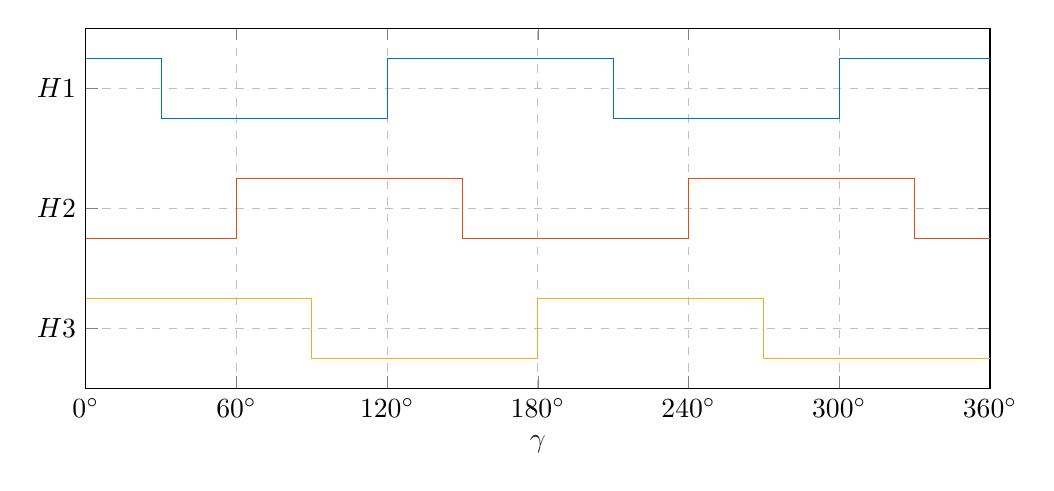
\begin{tikzpicture}

\begin{axis}[%
width=4.521in,
height=1.8in,
at={(0.758in,0.481in)},
scale only axis,
xmin=0,
xmax=360,
xtick={  0,  60, 120, 180, 240, 300, 360},
xticklabels={{$ 0^{\circ} $},  {$ 60^{\circ} $}, {$ 120^{\circ} $}, {$ 180^{\circ} $}, {$ 240^{\circ} $}, {$ 300^{\circ} $}, {$ 360^{\circ} $}},
xlabel style={font=\color{white!15!black}},
xlabel={$\gamma$},
ymin=-1,
ymax=11,
ytick={1,5,9},
yticklabels={{$ H3 $},{$ H2 $},{$ H1 $}},
axis background/.style={fill=white},
xmajorgrids,
ymajorgrids,
major grid style={dashed}
]
\addplot[const plot, color=mycolor1, forget plot] table[row sep=crcr] {%
0	10\\
30	8\\
60	8\\
90	8\\
120	10\\
150	10\\
180	10\\
210	8\\
240	8\\
270	8\\
300	10\\
330	10\\
360	10\\
};
\addplot[const plot, color=mycolor2, forget plot] table[row sep=crcr] {%
0	4\\
30	4\\
60	6\\
90	6\\
120	6\\
150	4\\
180	4\\
210	4\\
240	6\\
270	6\\
300	6\\
330	4\\
360	4\\
};
\addplot[const plot, color=mycolor3, forget plot] table[row sep=crcr] {%
0	2\\
30	2\\
60	2\\
90	0\\
120	0\\
150	0\\
180	2\\
210	2\\
240	2\\
270	0\\
300	0\\
330	0\\
360	0\\
};
\end{axis}
\end{tikzpicture}%
	\caption{Signale der Hallsensoren bei $ Z_{P} = 2 $}
	\label{fig:3a:hall}
\end{figure}

\section{}\label{sec:3b}
Gesucht ist nun ein Verfahren, mit dem man die Polpaarzahl eines BLDC bestimmen kann. Um die Polpaarzahl zu erhalten, können wir auch die positiven Flanken des Signals eines Hallsensors während einer Umdrehung des Rotors zählen.

